\documentclass[tikz,border=10pt]{standalone}
\usepackage{tikz}
\usetikzlibrary {angles,quotes,arrows.meta, intersections, calc}
\usepackage{tkz-euclide} %for right angle marker
\usetikzlibrary{decorations.markings}
\tikzset{%
  ->-/.style={decoration={markings, mark=at position 0.9 with {\arrow{>}}},
              postaction={decorate}},
  ->>-/.style={decoration={markings, mark=at position 0.9 with {\arrow{>>}}},
               postaction={decorate}},
}


\begin{document}
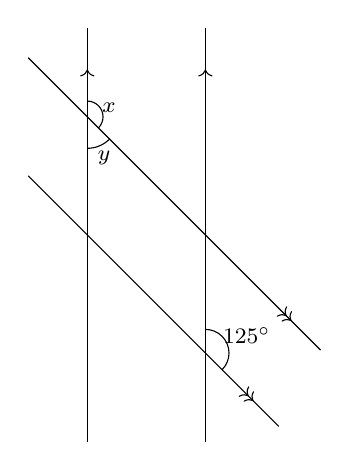
\begin{tikzpicture}[scale = 1.5]

% Draw first line at 55 degrees anticlockwise from the vertical
\draw[->>-, name path = leg] (0,0) -- ++(-45:3cm) coordinate (D); % 180 - 55 = 125 degrees

% Draw second line parallel to the first, at a distance
\draw[->>-, name path = leg1] ([shift={(0,1)}]0,0) -- ++(-45:3.5cm) coordinate (E);

% Draw vertical lines
% First vertical line
\draw[->-, name path=AK] ([shift={(0.5, -2.25)}]0,0) -- ++(90:3.5cm) coordinate (K);

% Second vertical line, placed to the right of the first
\draw[->-, name path = BM] ([shift={(1.5, -2.25)}]0,0) -- ++(90:3.5cm) coordinate (M);

\draw[name intersections={of=AK and leg1,by={C}}];
\draw[name intersections={of=AK and leg,by={G}}];
\draw[name intersections={of=BM and leg,by={H}}];

% Draw the angle between lines
    \pic [draw, "\footnotesize $x$ ", angle eccentricity=1.5, angle radius=0.2cm] {angle = E--C--K};
    \pic [draw, "\footnotesize $y$ ", angle eccentricity=1.4, angle radius=0.4cm] {angle = G--C--E};
    \pic [draw, "\footnotesize $125^\circ$ ", angle eccentricity=1.9, angle radius=0.3cm,] {angle = D--H--M};

\end{tikzpicture}
\end{document}


